\documentclass[tikz,border=5pt]{standalone}
\usepackage{tikz}
\usepackage{amsmath}
\begin{document}

\begin{figure}[h]
\begin{center}
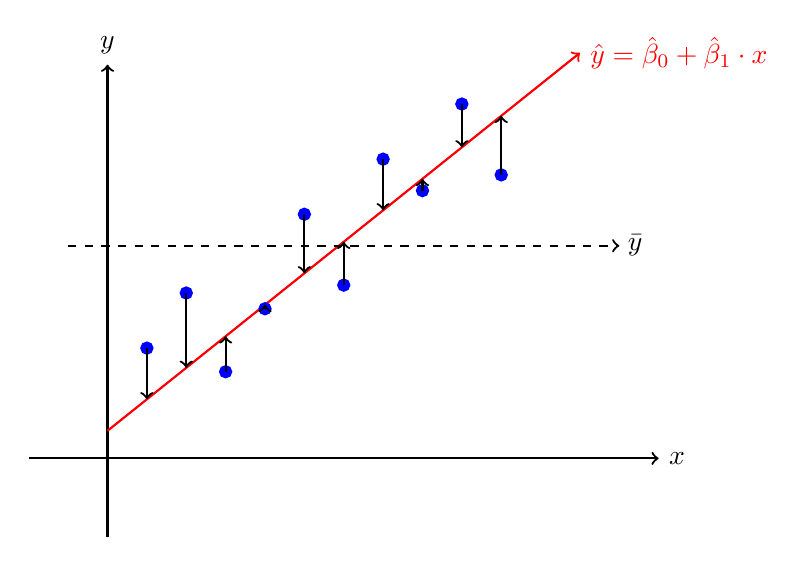
\begin{tikzpicture}[->, thick]
  \draw[->] (-1,0) -- (7,0) node[right] {$x$};
  \draw[->] (0,-1) -- (0,5) node[above] {$y$};
  \draw[red, thick, domain=0:6] plot (\x, {0.8*\x + 0.35}) node[right] {$\hat{y} = \hat{\beta}_0 + \hat{\beta}_1 \cdot x$};
  \filldraw[blue] (0.5, 1.4) circle (2pt);
  \filldraw[blue] (1.5, 1.1) circle (2pt);
  \filldraw[blue] (1, 2.1) circle (2pt);
  \filldraw[blue] (2, 1.9) circle (2pt);
  \filldraw[blue] (2.5, 3.1) circle (2pt);
  \filldraw[blue] (3, 2.2) circle (2pt);
  \filldraw[blue] (3.5, 3.8) circle (2pt);
  \filldraw[blue] (4, 3.4) circle (2pt);
  \filldraw[blue] (4.5, 4.5) circle (2pt);
  \filldraw[blue] (5, 3.6) circle (2pt);
  \foreach \x/\y in {
    0.5/1.4, 
    1.5/1.1,
    1/2.1,
    2/1.9,
    2.5/3.1,
    3/2.2,
    3.5/3.8,
    4/3.4,
    4.5/4.5,
    5/3.6
  }{
    \draw[black] (\x,\y) -- (\x,{0.8*\x + 0.35});
  }
  \draw[dashed] (-0.5,2.7) -- (6.5,2.7);
  \node at (6.7,2.7) {$\bar{y}$};
\end{tikzpicture}
\end{center}
\caption{A simple linear regression illustration with residuals shown. Blue points are observed data, red line is the model, dashed line is the average of $y$, and black lines represent residuals $y_i - \hat{y_i}$.}
\end{figure}

\end{document}